\documentclass[11pt]{article}

\usepackage[T1]{fontenc}
\usepackage[utf8]{inputenc}
\usepackage[pdfusetitle]{hyperref}
\usepackage{graphicx}
\usepackage{float}
\usepackage[MeX]{polski}
\usepackage{tabularx}
\usepackage[a4paper,left=3cm,right=3cm,top=2.5cm,bottom=2.5cm]{geometry}
\usepackage{titlesec}
\usepackage{indentfirst}
\usepackage{hyperref}
\usepackage[normalem]{ulem}
\usepackage{secdot}

\title{Specyfikacja karaoke-app}
\author{Grupa F}

\begin{document}
  \maketitle

  \section{Wprowadzenie}
  Aplikacja \textit{karaoke-app} ma za zadanie udostępnienie popularnej rozrywki, jaką jest Karaoke, poprzez wygodny i intuicyjny interfejs dostępny z poziomu przeglądarki internetowej. Użytkownik wybiera utwór spośród dostępnych w katalogu, lub dodaje nowy poprzez wizualny kreator dostępny dla zalogowanych użytkowników. Podczas odtwarzania utworu wyświetlany jest tekst z wyróżnioną aktualną linią do zaśpiewania (według czasu).

  \section{Zespół}
  \begin{itemize}
    \item Dawid Bury (tester)   
    \item Daniel Hajduk (frontend developer)
    \item Adrian Korczykowski (dev-ops)
    \item Łukasz Poterała (backend developer)
    \item \underline{Mariusz Zdancewicz} (PM/frontend developer)
  \end{itemize}

  \section{Technologia}
  
  \begin{itemize}
    \item Backend
    \begin{itemize}
      \item PHP >= 7.2
      \item Laravel 6.x
      \item MySQL >= 5.6
    \end{itemize}
    \item Frontend
    \begin{itemize}
      \item Vue 2.x
    \end{itemize}
  \end{itemize}

  Aplikacja kliencka przystosowana jest do działania z najnowszymi wersjami przeglądarek Chrome i Firefox, także na urządzeniach mobilnych.

  \section{Role}
  Przewiduje się trzy podstawowe role w systemie:

  \begin{itemize}
    \item gość (osoba anonimowa, niezalogowana do systemu),
    \item zalogowany użytkownik,
    \item administrator.
  \end{itemize}

  \section{Funkcjonalności}
  Aplikacja powinna implementować następujący szereg funckjonalności.

  \subsection{Uwierzytelnianie użytkowników}
  Użytkownik może zarejestrować się w systemie podając podstawowe dane takie jak nazwa użytkownika, adres email i hasło. Konto zostanie aktywowane po pomyślnym potwierdzeniu adresu email poprzez wejście w wysłany link aktywacyjny. Po aktywowaniu konta użytkownik może skorzystać z formularza logowania.

  Oprócz tradycyjnego modelu rejestracji i logowania przewiduje się możliwość logowania za pomocą wybranych serwisów social media: Facebooka i Google.

  \subsection{Kreator utworów}
  Kreator utworów jest funkcjonalnością dostępną tylko dla zalogowanych użytkowników. Użytkownik może skorzystać z wizualnego kreatora utworu w celu dodania własnego utworu do bazy danych. Kreator podzielony jest na 2 etapy:

  \begin{enumerate}
    \item synchronizacja tekstu utworu ze ścieżką dźwiękową,
    \item wprowadzanie metadanych utworu.
  \end{enumerate}

  W pierwszym etapie użytkownik importuje wideo z dwóch dostępnych serwisów wideo (Youtube lub Vimeo), wprowadza tekst utworu z podziałem na linie, a następnie oznacza czasy rozpoczęcia i zakończenia danych linii tekstu.

  W etapie drugim wprowadzane są metadane utworu takie jak jego tytuł, artysta czy przynależność do kategorii.

  \begin{figure}[ht]
    \centering
    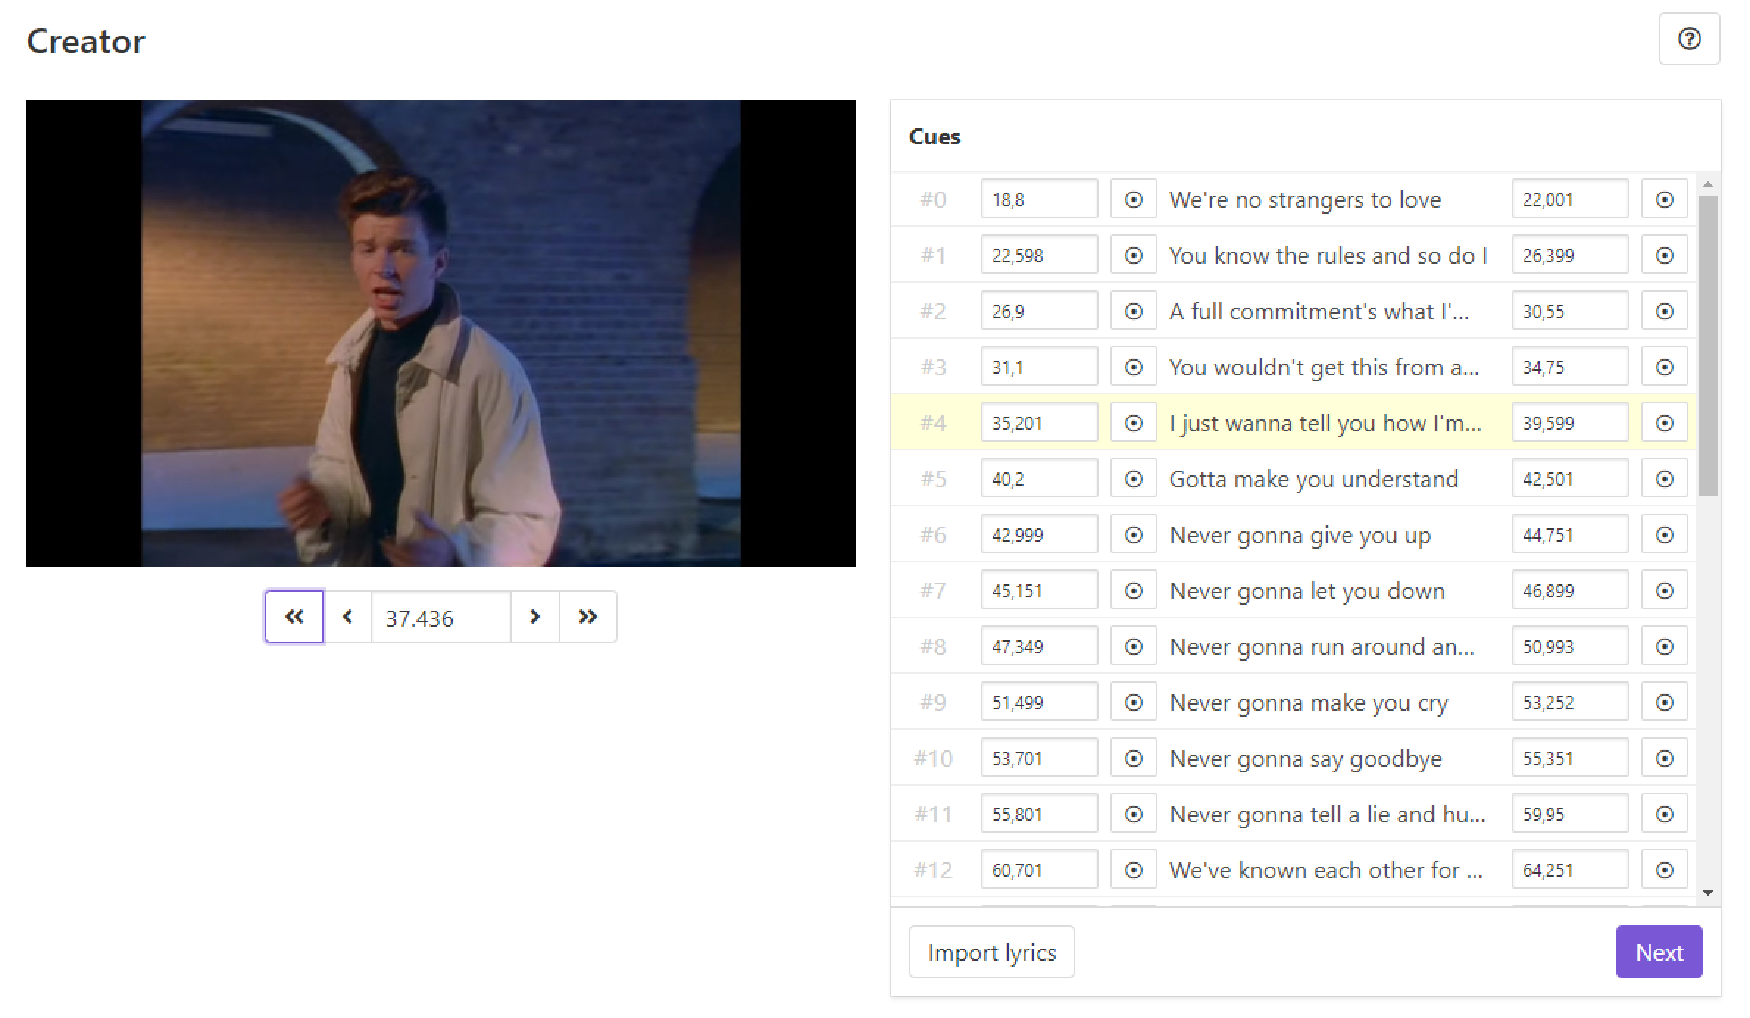
\includegraphics[width=1.0\textwidth]{sample-creator.pdf}
    \caption{Przykładowy interfejs kreatora}
  \end{figure}

  \subsection{Katalog utworów}
  Katalog utworów podzielony jest na kategorie definiowane przez administratora systemu. Utwór może być przypisany do wielu kategorii. Użytkownik ma możliwość filtrowania listy utworów poprzez wybór kategorii oraz sortowanie według czasu dodania utworu lub po nazwie (alfabetycznie).

  Ponadto użytkownik może skorzystać z wyszukiwarki utworów (podając tytuł i/lub artystę).

  \subsection{Utwór}
  Widok utworu zawiera moduł karaoke oraz wyświetla podstawowe informacje o utworze (takie jak tytuł, arysta, data utworzenia, ocena czy liczba wyświetleń). Ponadto wyświetlane są podpowiedzi innych utworów (np. inne utwory tego samego artysty lub inne utwory utworzone przez użytkownika).

  \subsubsection{Moduł karaoke}
  W głównym module aplikacji, module karaoke, wyświetlane jest wideo utworu wraz z aktualną i następną linią tekstu do odśpiewania. Moduł można uruchomić w trybie pełnoekranowym, zmieniać wielkość tekstu a także resetować utwór.

  \begin{figure}[ht]
    \centering
    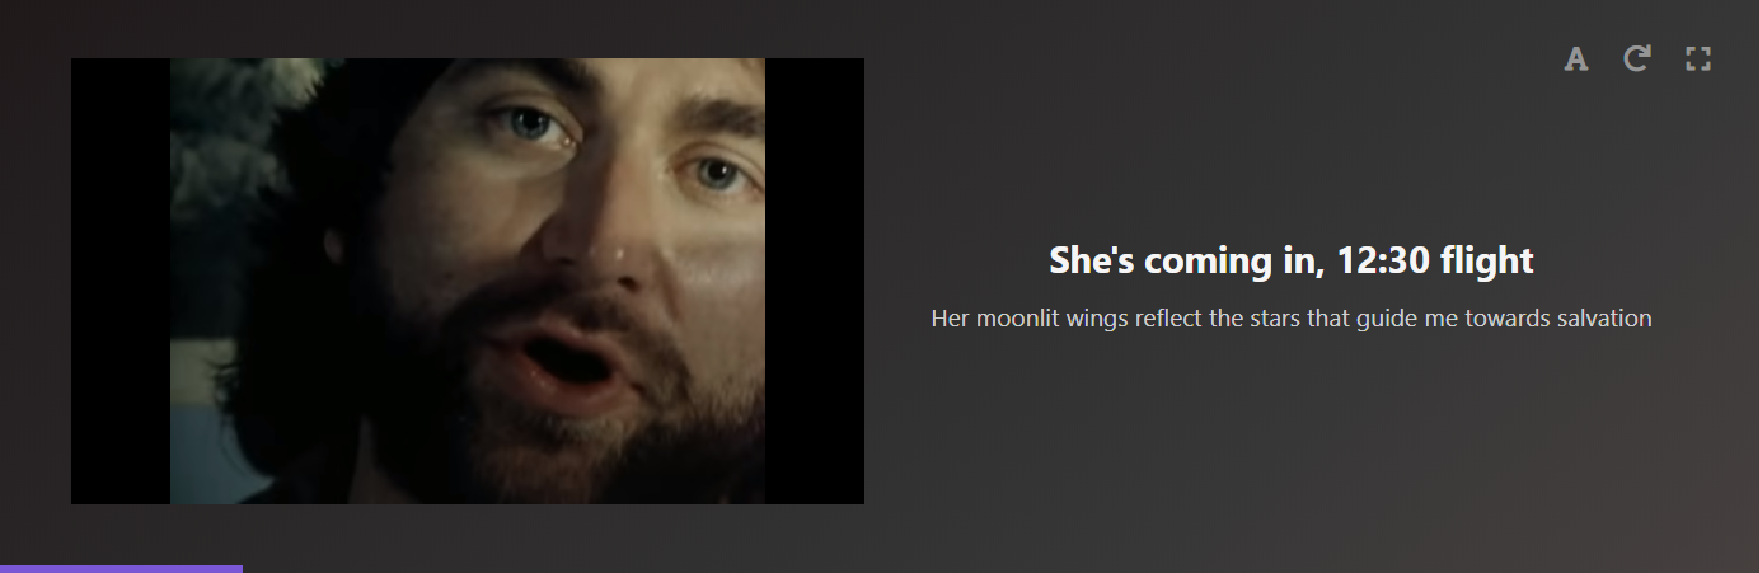
\includegraphics[width=1.0\textwidth]{sample-karaoke_module.pdf}
    \caption{Przykładowy interfejs modułu karaoke}
  \end{figure}

  \subsubsection{Ocena}
  Zalogowany użytkownik ma możliwość oceny utworu w skali od 1 do 5.

  \subsubsection{Zgłaszanie problemów}
  Zalogowany użytkownik ma możliwość wysłania zgłoszenia problemu związanego z utworem do administratora (np. niedziałające wideo czy błędna synchronizacja tekstu).

  \subsection{Profil użytkownika}
  Każdy użytkownik systemu posiada swój profil, na którym dostępne są następujące informacje:

  \begin{itemize}
    \item podstawowe dane o użytkowniu (jego nazwa),
    \item utworzone playlisty (mając na uwadze ustawienia prywatności),
    \item utwory stworzone przez użytkownika.
  \end{itemize}

  Ponadto jeśli użytkownik jest zalogowany i odwiedza swój własny profil, dostępna jest dla niego konfiguracja konta:

  \begin{itemize}
    \item zmiana nazwy użytkownika,
    \item zmiana hasła,
    \item deaktywacja konta.
  \end{itemize}

  \subsection{Playlisty}
  Zalogowani użytkownicy mogą tworzyć tzw. \textit{playlisty}, czyli własne listy utworów skomponowane z utworów dostępnych w aplikacji. Po odtworzeniu playlisty utwory na niej przełączane są automatycznie. Do wyboru są dwa tryby przełączania:
  \begin{enumerate}
    \item "jeden po drugim" (tryb standardowy),
    \item tryb losowy.
  \end{enumerate}
  
  Playlista może zostać oznaczona jako prywatna, wówczas będzie widoczna jedynie dla użytkownika, który ją utworzył. Domyślnie playlisty są publiczne.

  \subsection{Panel adminstratora}
  Administrator ma możliwość skorzystania z dedykowanego panelu do monitorowania i modyfikowania działania aplikacji. Dostępne są dla niego funkcje:

  \begin{itemize}
    \item zarządzanie użytkownikami,
    \item zarządzanie utworami (w tym weryfikowanie utworów dodanych przez kreator),
    \item zarządzanie kategoriami.
  \end{itemize}

  \subsection{Analiza ruchu}
  Analiza ruchu w aplikacji odbywa się poprzez:
  
  \begin{itemize}
    \item logowanie podstawowych zdarzeń (takich jak zalogowanie do systemu, utworzenie nowego konta, utworzenie utworu za pomocą kreatora czy utworzenie nowej playlisty),
    \item licznik odtworzeń poszczególnych utworów,
    \item skorzystanie z usługi \textit{Google Analytics}.
  \end{itemize}
\end{document}